\frametitle{Docking results of Ethotoin}
\begin{columns}
	\begin{column}{0.6\linewidth}
		\begin{figure}
			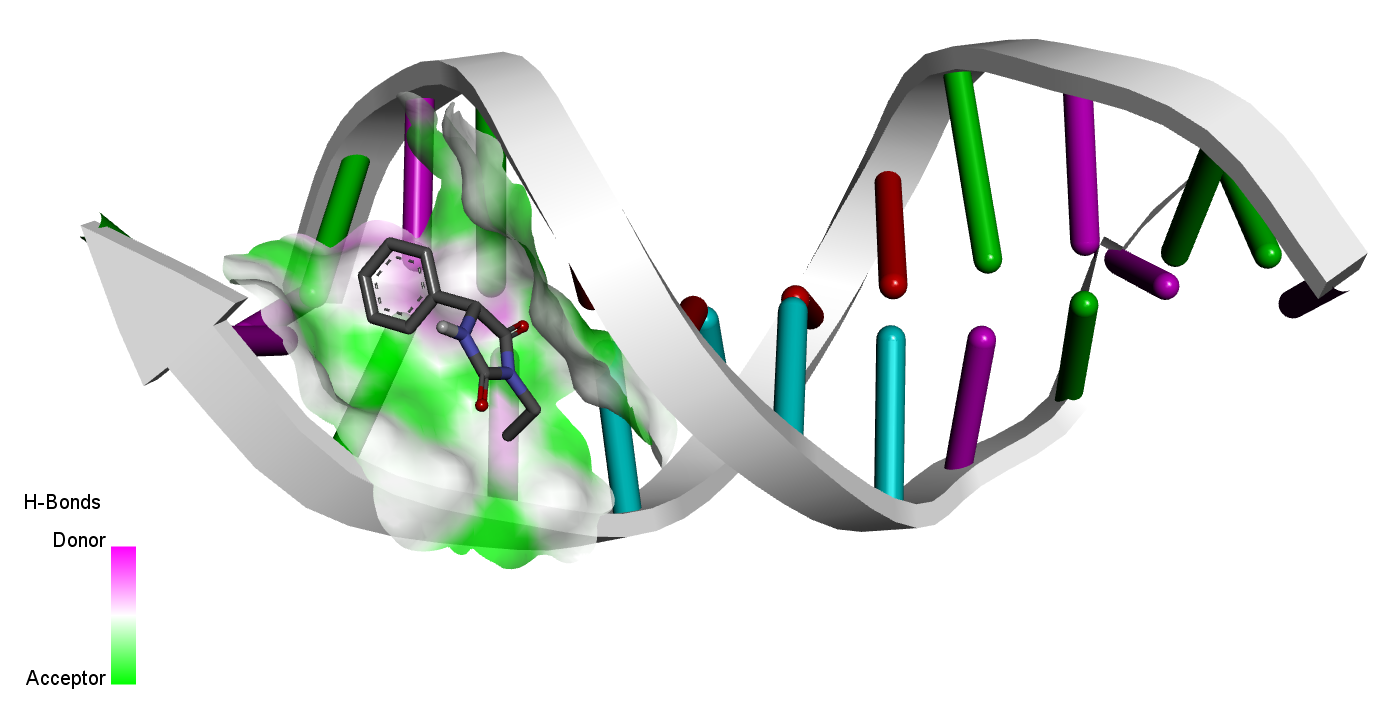
\includegraphics[width=\linewidth]{ethotoin-donor-acceptor.png}
			\caption{\centering The donor-acceptor interaction \linebreak between Ethotoin and B-DNA.}
			\label{fig:eth_donor_acceptor}
		\end{figure}
	\end{column}
	\begin{column}{0.45\linewidth}
		\centering
		\scriptsize
		\begin{table}
			\begin{tabular}{*{4}{c}}
				\hline\\[-1em]
				\multirow{2}{2em}{\centering\textbf{Mode}}&\multirow{2}{4em}{\centering\textbf{Affinity (kcal/mol)}}&\multicolumn{2}{c}{\centering\textbf{Distance from best mode}}\\
				\cline{3-4}
				&&\textbf{rmsd l.b.}&\textbf{rmsd u.b.}\\
				1&-5.8&0.000&0.000\\
				2&-5.7&2.861&5.332\\
				3&-5.7&2.603&4.023\\
				4&-5.7&1.849&5.310\\
				5&-5.7&1.750&5.199\\
				6&-5.6&2.236&5.225\\
				7&-5.4&2.600&4.039\\
				8&-5.4&3.081&5.706\\
				9&-5.3&1.431&2.061\\
				\hline
			\end{tabular}
			\caption{\centering The binding affinities and RMSD values \linebreak between Ethotoin and B-DNA.}
			\label{table:eth}
		\end{table}
	\end{column}
\end{columns}